\chapter{User Interface}


\subsection{Log in to the web portal}
\begin{figure}[h]
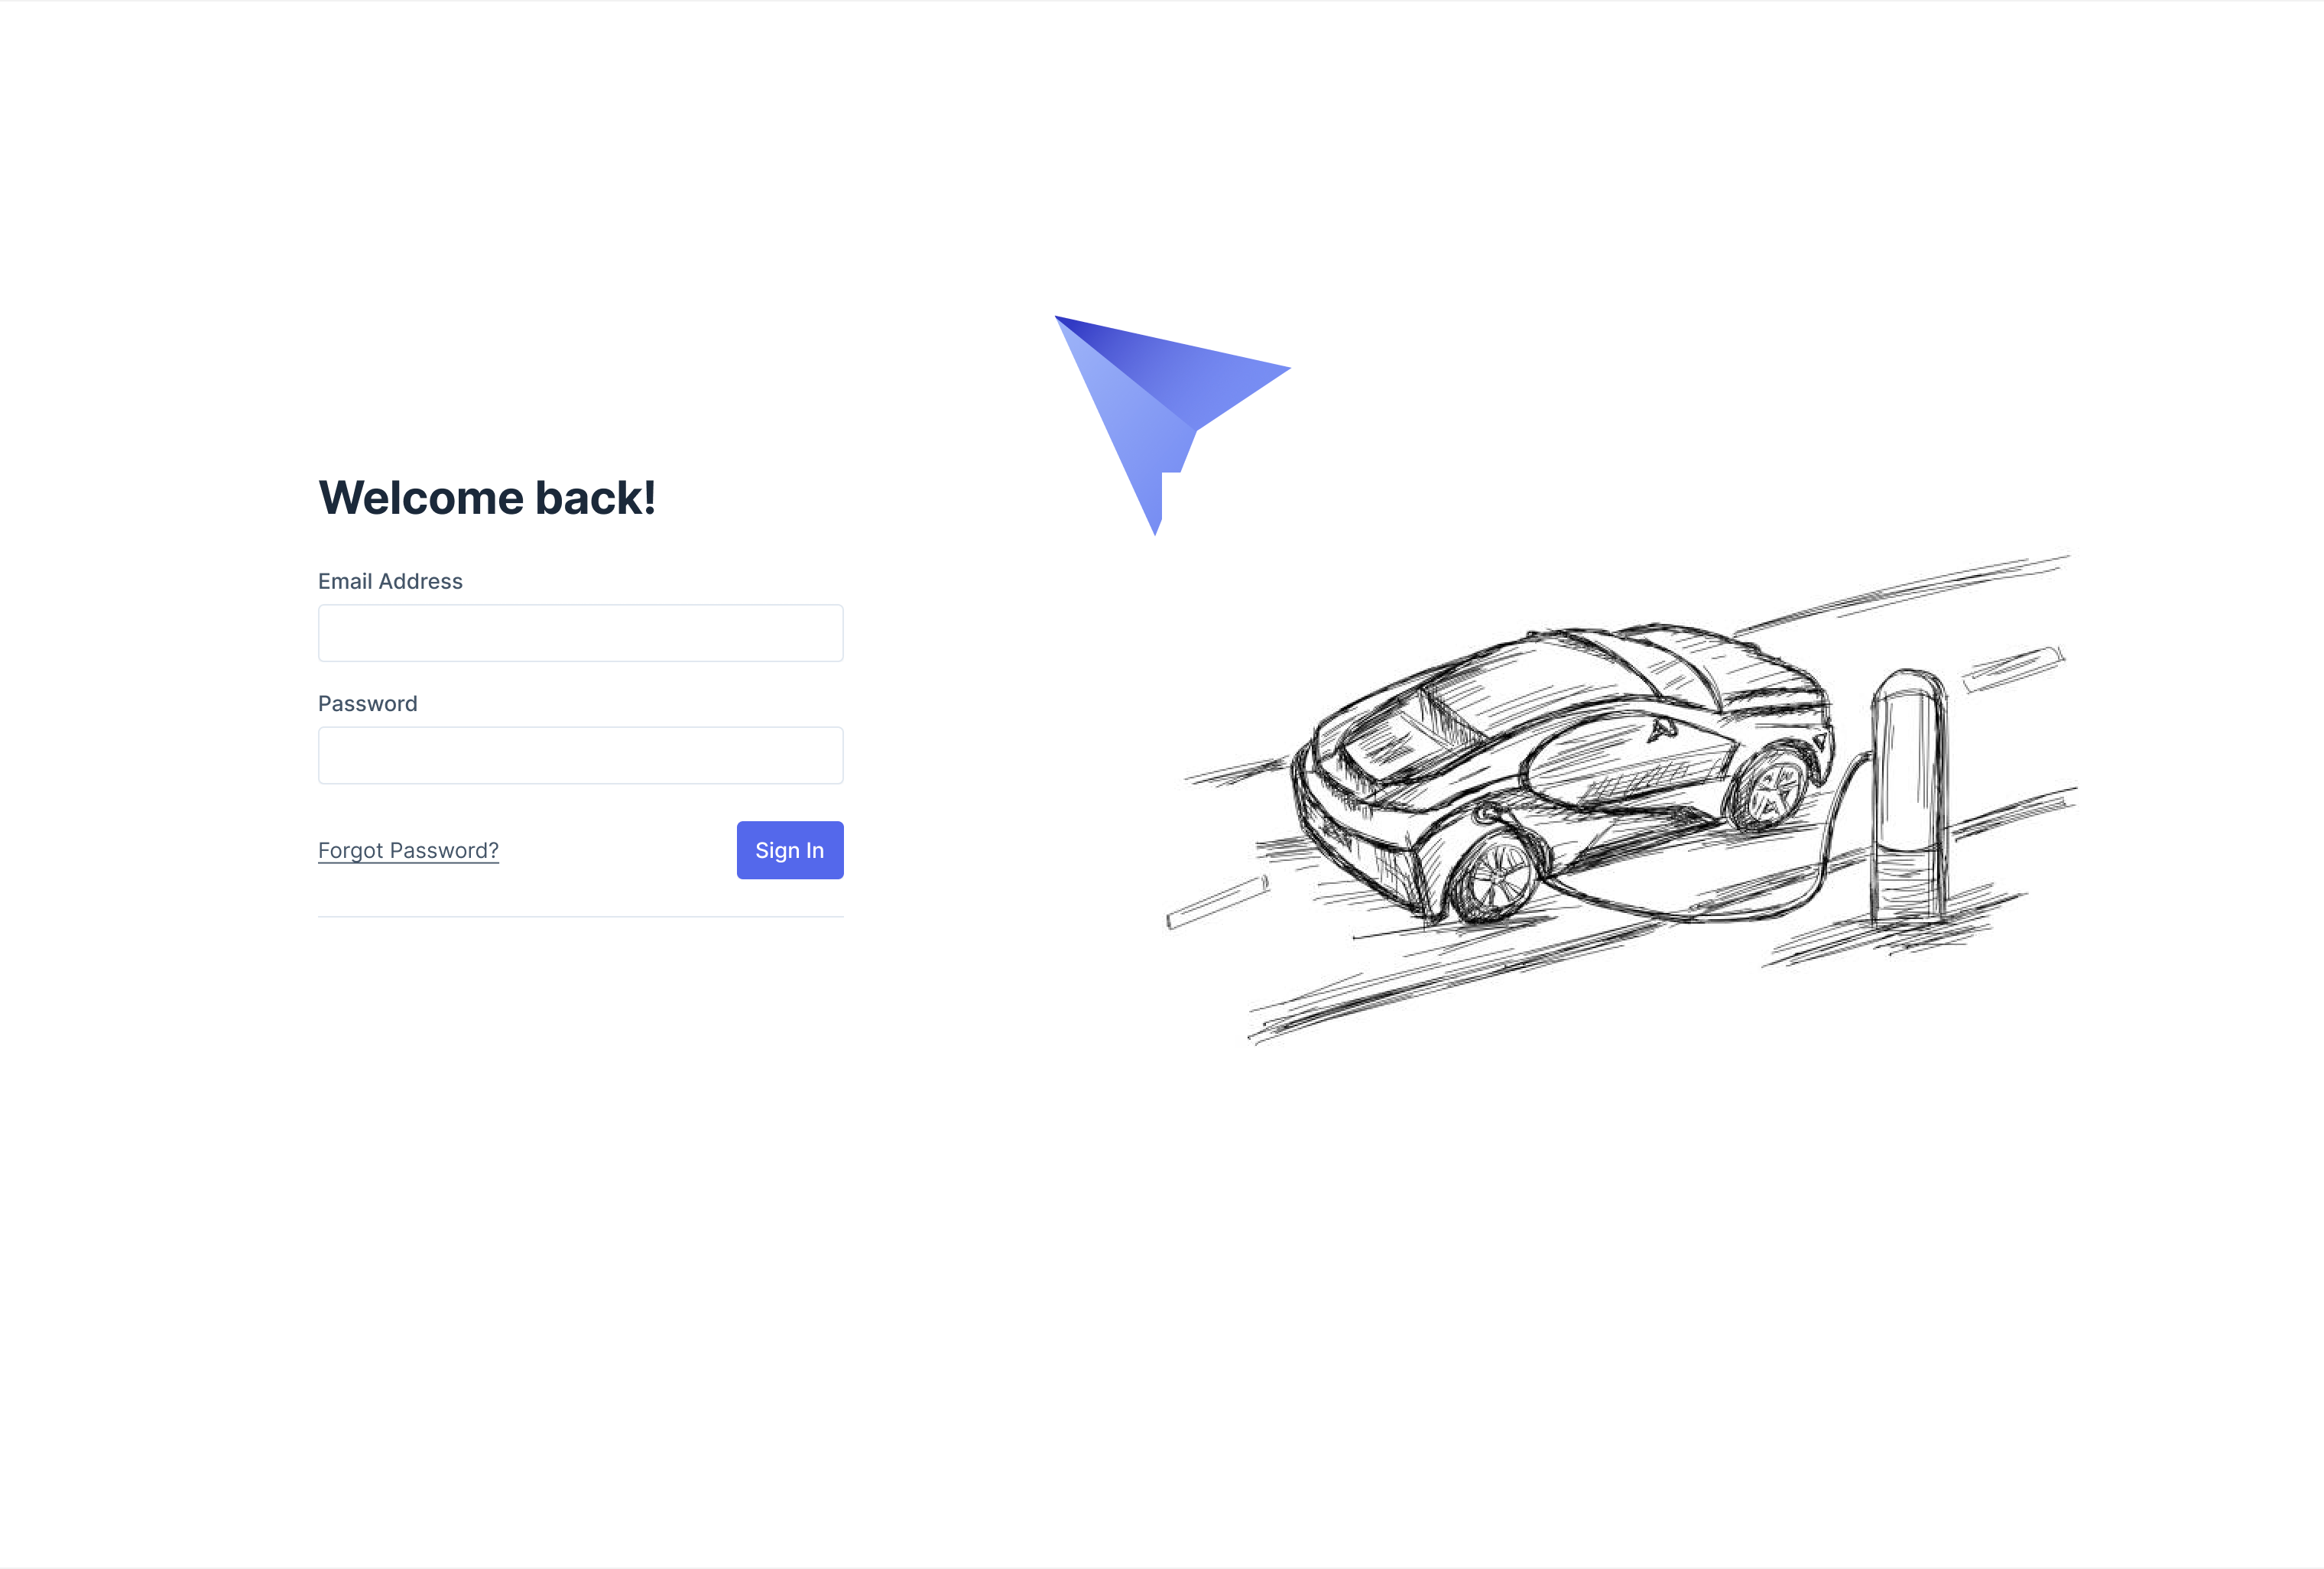
\includegraphics[width=11cm]{UI/login}
\caption{Log in to the web portal}
\end{figure}
In this first view, the user opens the site hosted by his own CPMS, and enters his credentials to access the pages dedicated to him.

\pagebreak

\subsection{View energy sources report}
\begin{figure}[h]
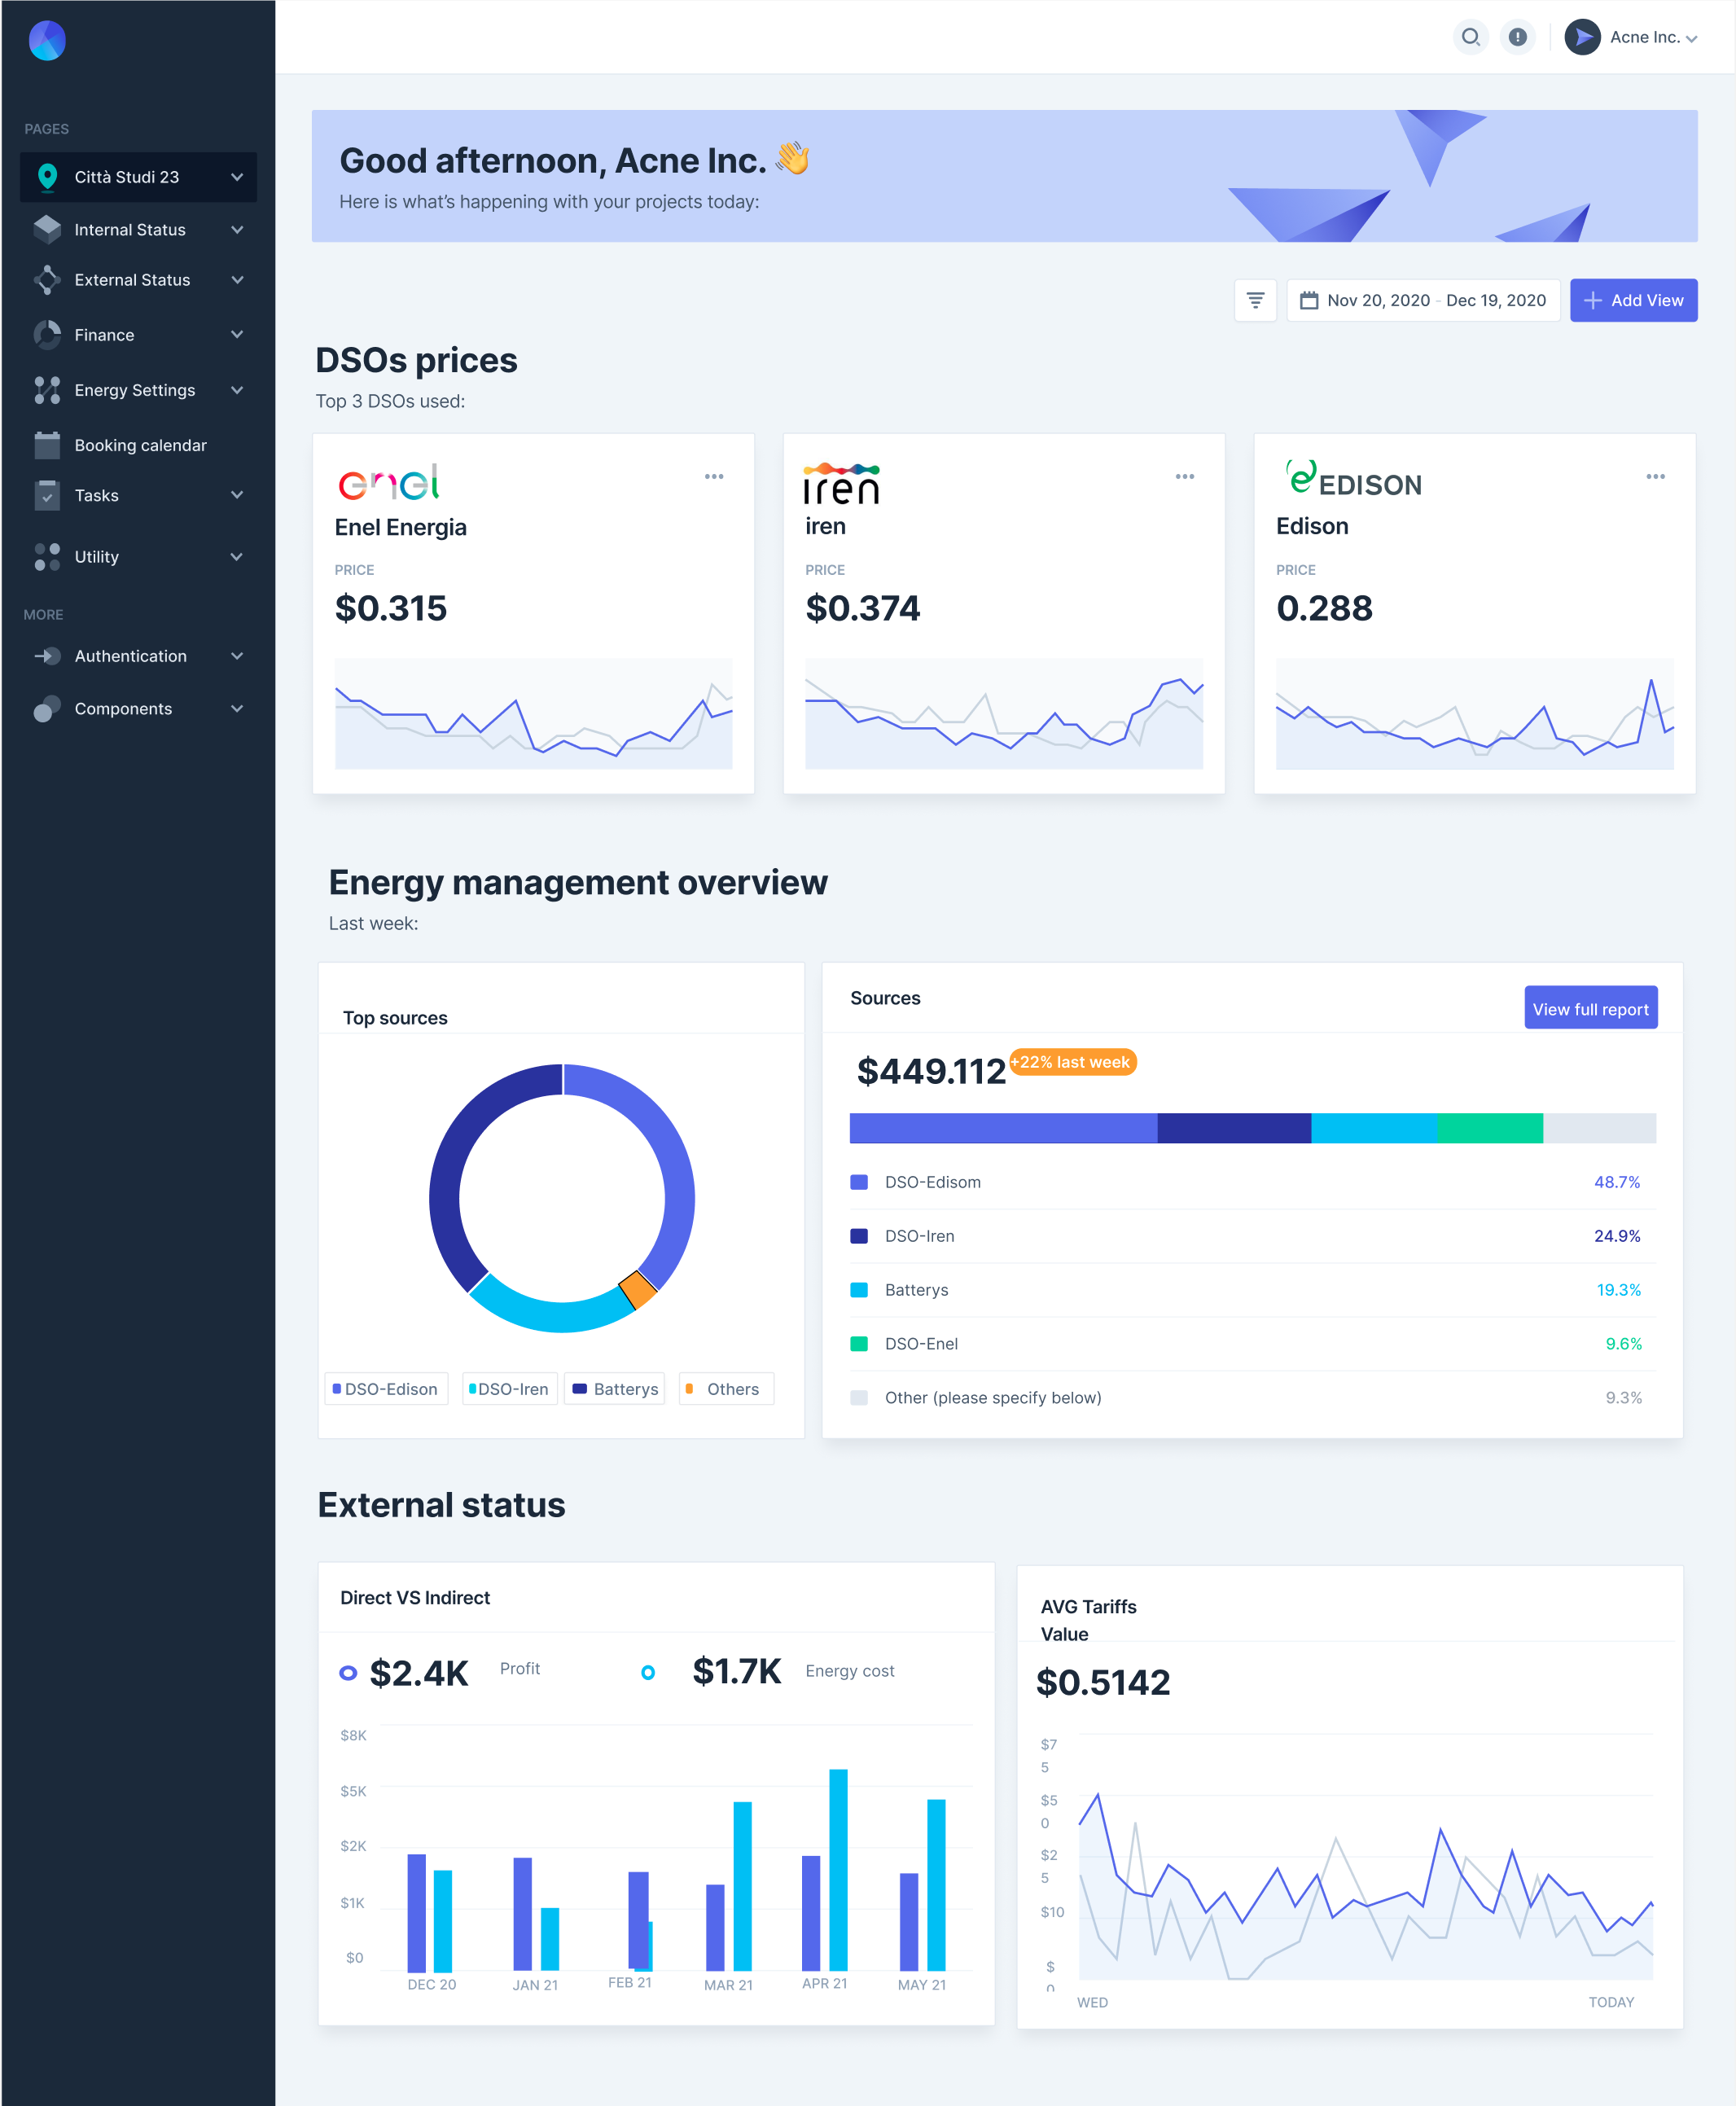
\includegraphics[width=11cm]{UI/Dashboard}
\caption{View energy sources report}
\end{figure}
The CPO administrator wants to view the report regarding the energy sources used during the last month. Then access the portal using your credentials. Then select the relevant charging station, using the drop-down menu on the left. Then press the "View full report" button. The site will display a file containing the requested data.\\


\pagebreak
\subsection{View external status informations}
\begin{figure}[h]
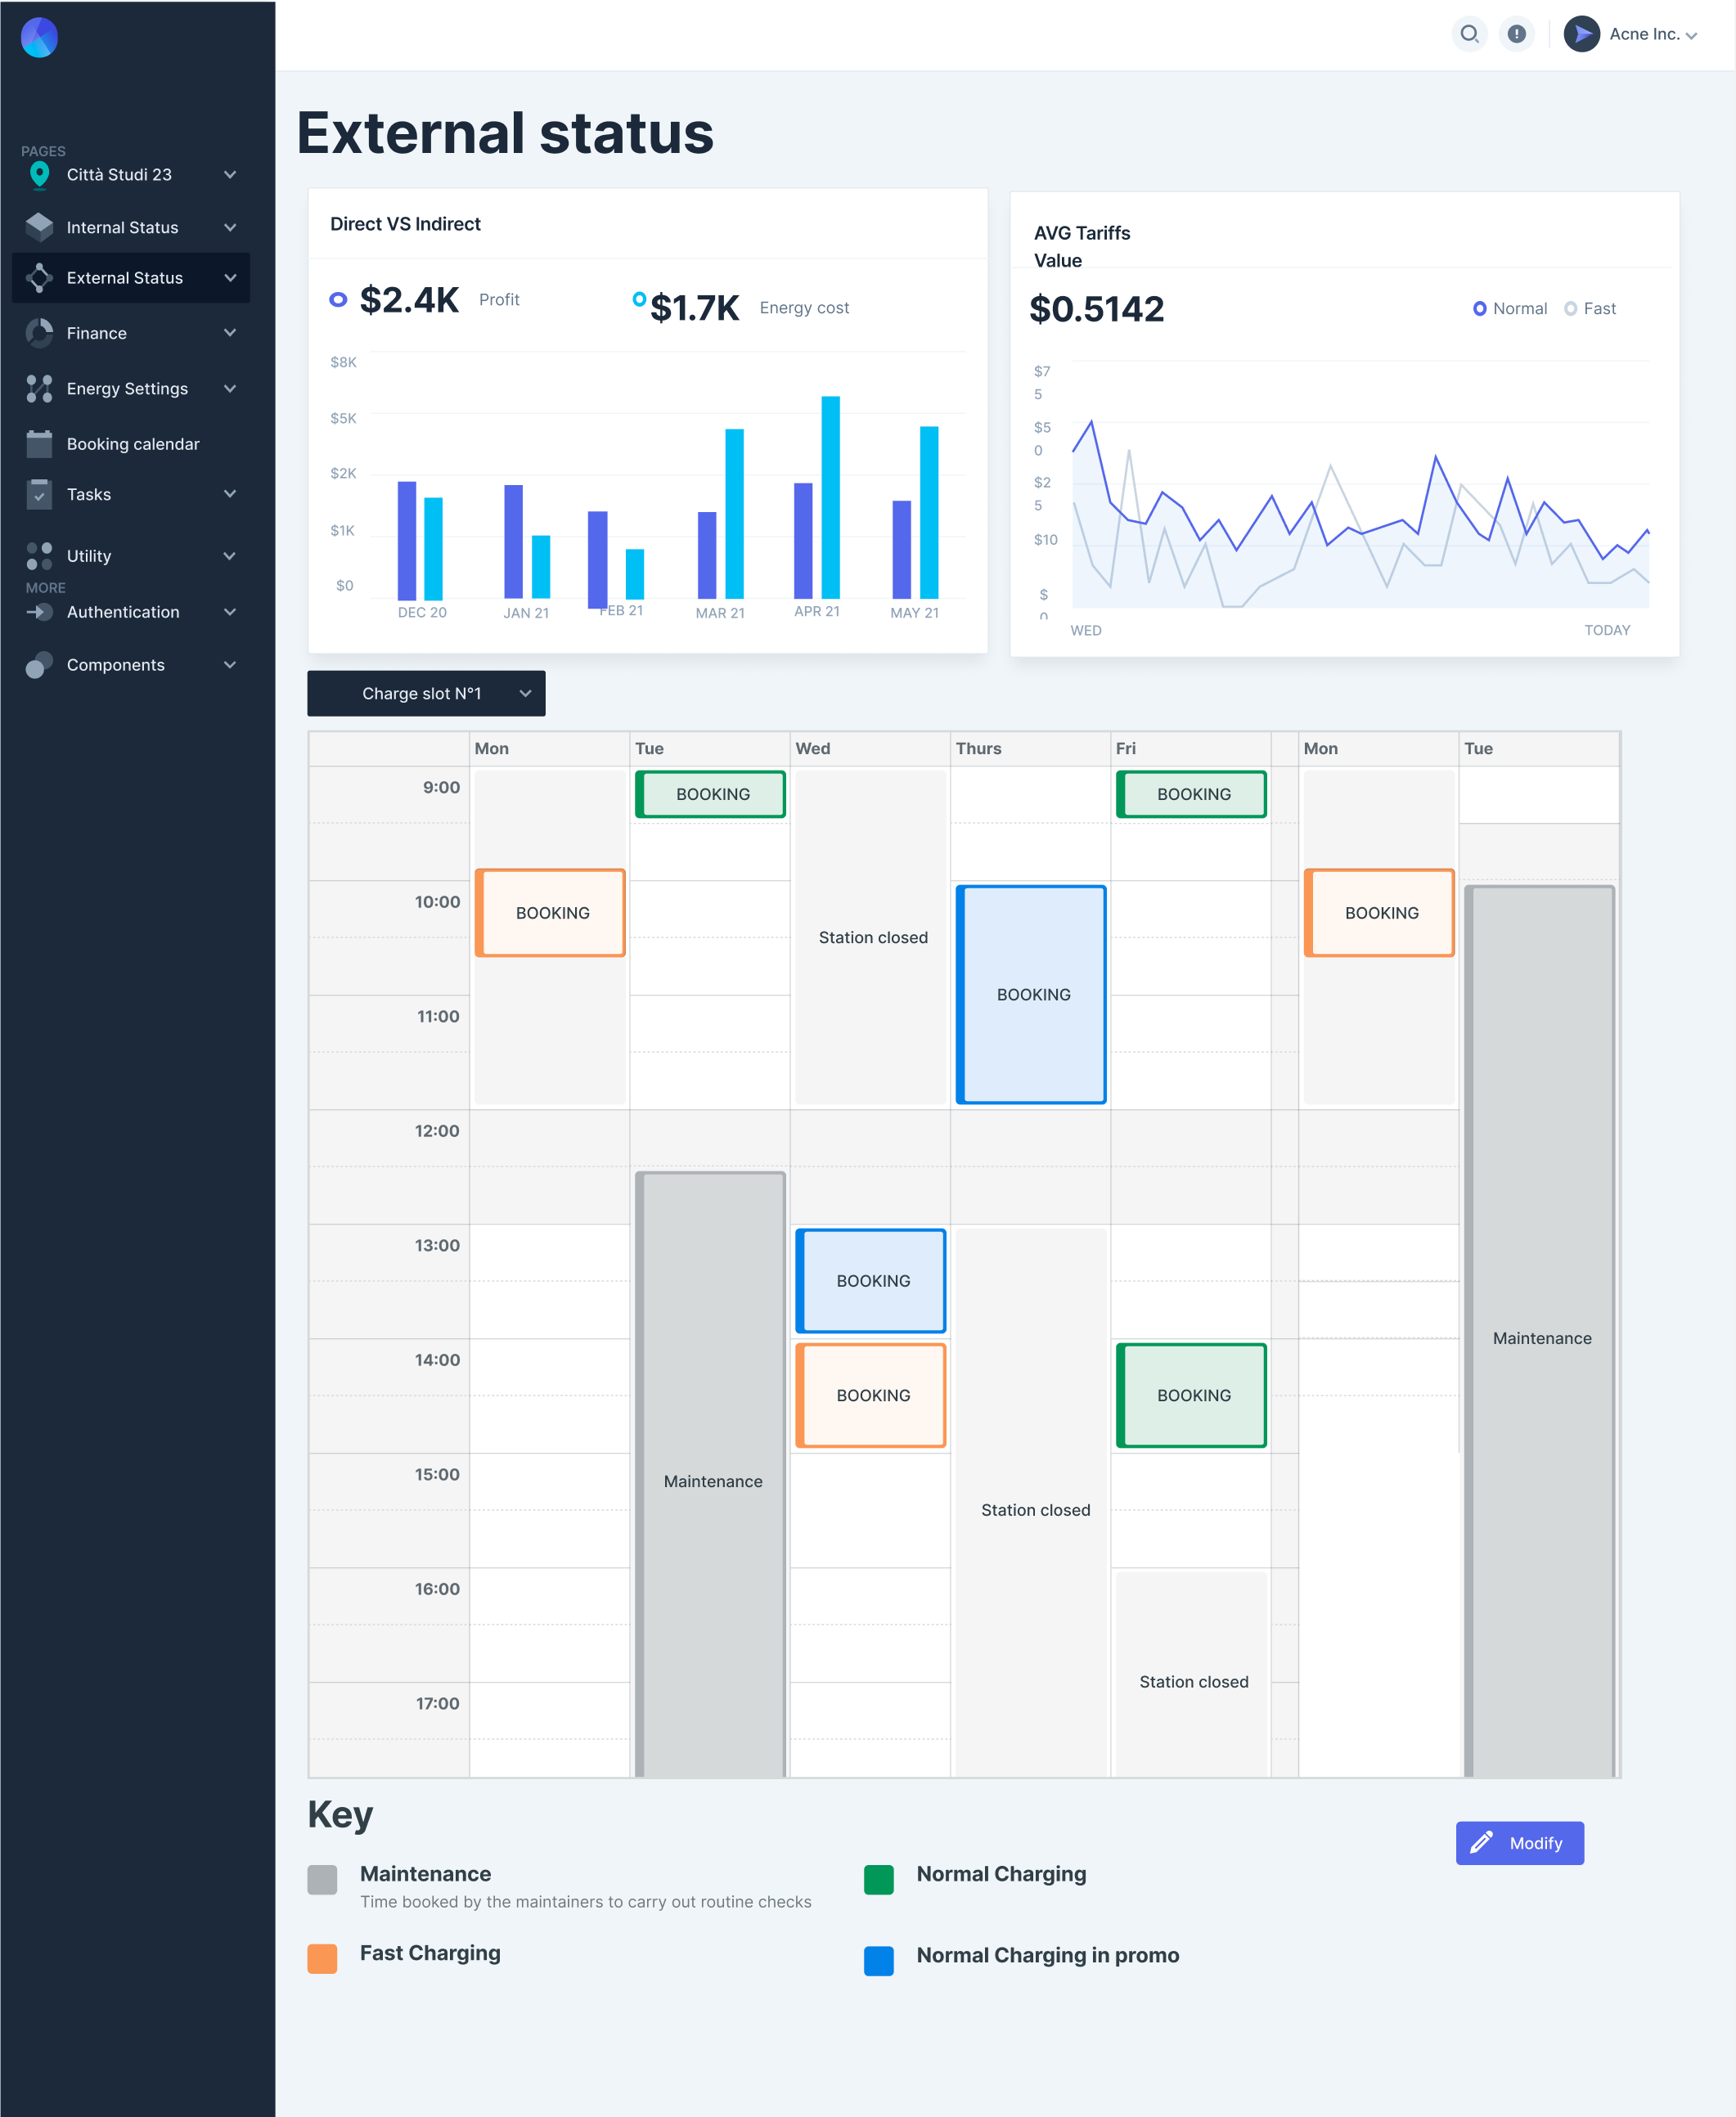
\includegraphics[width=11cm]{UI/External_status}
\caption{View external status informations}
\end{figure}
The CPO wants to view information regarding the external status of one of its charging stations. He then accesses the portal using his credentials and selects the Charging station using a special drop-down menu located on the left. After that select the "External status" page. The page containing all the information regarding the external status will then be displayed.
\clearpage
